\documentclass[11pt]{article}
\usepackage{amsmath,amssymb,amsthm,enumerate,nicefrac,fancyhdr,hyperref,graphicx,adjustbox}
\hypersetup{colorlinks=true,urlcolor=blue,citecolor=blue,linkcolor=blue}
\usepackage[left=2.6cm, right=2.6cm, top=1.5cm, includehead, includefoot]{geometry}
\usepackage[dvipsnames]{xcolor}
\usepackage[d]{esvect}
\usepackage{listings}
\usepackage{enumitem} % To allow for alph in enumerate
\usepackage{braket}
\usepackage{float} % To allow for H setting in figures.

% to draw dfas
\usepackage{tikz}
\usetikzlibrary{automata, positioning, arrows}


%% header
\pagestyle{fancy}
\fancyhead[L]{\bf\large CSC236 UTM \\ Assignment 3}
\fancyhead[R]{\bf\large Fall 2024  \\Due Nov 25}
%\fancyfoot[C]{Page \thepage\ of 2}
\setlength{\headheight}{35pt}

\begin{document}
\tikzset{
->, % makes the edges directed
>=stealth', % makes the arrow heads bold
node distance=3cm, % specifies the minimum distance between two nodes. Change if necessary.
every state/.style={thick, fill=gray!10}, % sets the properties for each ’state’ node
initial text=$ $, % sets the text that appears on the start arrow
}

You are not allowed to post the assignment questions anywhere; however, you are allowed to search the internet (just cite your resources if you find any). You are also allowed to bounce ideas off classmates and TAs, but at the end, you must write your own solutions. 

If you use AI tools, please mention the name of the tool and the prompts you used.

\vspace{0.2cm}


%\vspace{0.3cm}

	\begin{enumerate}[label=\textbf{Q\arabic*.}]


%%%%%%% Q1
\item \textbf{(18 pts)}

Show with proof which of the following languages is regular and which is not. If you show that a language is regular, you are expected to provide a DFA that accepts the language. 

Let $ \Sigma = \{0,1\} $.

\begin{enumerate}[label=\textit{\alph*)}]
	\item \textbf{(3 pts)} $ \Sigma^* $
	
	\begin{proof}
		From the definition of a regular language, \(\{ 0 \} \) and \(\{ 1 \} \) are regular languages. Then \(\{ 0 \} \cup \{ 1 \} = \Sigma\) is a regular language. Finally, it is true that \(\Sigma ^*\) is a regular language.

		For this regular language, define the DFA \(\mathcal{D} = (\{q_0\}, \Sigma, \delta , q_0, \{q_0\})\), where \(\delta : \{q_0\} \times \Sigma \to \{q_0\}\) is a function that always maps to \(q_0\).
		
		\begin{figure}[ht]
			\centering
			\begin{tikzpicture}
				\node[state,initial,accepting] (q0) {q0};
				\draw (q0) edge[loop above] node{0} (q0)
					  (q0) edge[loop below] node{1} (q0);
			\end{tikzpicture}
			\label{fig:DFA for a)}
		\end{figure}

	\end{proof}

	\item \textbf{(3 pts)} $ \Sigma^*\backslash\{K\}, K =\{01, 101, 010\}$
	
	\begin{proof}
		\begin{figure}
			\centering
			\begin{tikzpicture}
				\node[state,initial,accepting] (q0) {q0};
				\node[state, right of=q0] (q1) {q1};
			\end{tikzpicture}
			\label{DFA for b)}
		\end{figure}
	\end{proof}
	\item \textbf{(3 pts)} $ \{w \mid w \text{ is a palindrome}\} $
	
	\begin{proof}
		This is not regular. Suppose for contradiction that this languages was regular. Then there would be a DFA associated with this language. Let \(q\) be the number of states in this DFA, and let \(q_0\) denote the initial state. Define the following strings:
		\[
			w_i = 0^q 1 0^{i} \text{, for } i \in \{0, 1, 2, ..., q\}
		\]
		Notice that there are \(q+1\) strings in total. By the pigeonhole principle, at least 2 \(w_i, w_j\) will be in the same state \(q_c\), \(i < j\), that is, \(\delta (q_0, w_i) = \delta (q_0, w_j) = q_c\). It follows that \(\delta (q_0, w_i 0^{q-i}) = \delta (q_0, w_j 0^{q-i})\). But notice that
		\[
			w_i = 0^q 1 0^q \text{ and } w_j = 0^q 1 0^{q+j-i} \text{.} 
		\]
		It can be seen that \(w_i\) is a palindrome and should be accepted, but because \(q + j - i \neq q\), \(w_j\) is not a palindrome, which contradicts the fact that \(w_i\) and \(w_j\) are in the same state.

	\end{proof}
	\item \textbf{(3 pts)} $ \{ww \mid w \in \Sigma^*  \} $
	\item \textbf{(3 pts)} $ \{w \mid ww \in \Sigma^*  \} $

	\begin{proof}
		Denote the language above as \(A\). It will be shown that the language above is equivalent to \(\Sigma ^*\) using double subset inclusion.

		Trivially, \(A \subseteq \Sigma ^*\). Conversely, let \(w \in \Sigma ^*\). Then since \(ww \in \Sigma ^*\), \(w \in A\), proving the claim. Therefore, from part a), it can be concluded that \(A = \Sigma ^*\) is a regular language.

	\end{proof}
	\item \textbf{(3 pts)} $ \{w \mid w \text{ is a binary representation of a multiple of 3}\} $
	
	\begin{proof}
		Consider the following DFA:

		\begin{center}
			\begin{tikzpicture}
				\node[state,initial] (qi) {\(q_i\)};
				\node[state,right of=qi,accepting] (q0) {\(q_0\)};
				\node[state,right of=q0] (q1) {\(q_1\)};
				\node[state,right of=q1] (q2) {\(q_2\)};
				\draw (qi) edge[below] node{0} (q0)
						(qi) edge[bend left, above] node{1} (q1)
						(q0) edge[loop below] node{0} (q0)
						(q0) edge[above, bend left] node{1} (q1)
						(q1) edge[bend left, above] node{0} (q2)
						(q1) edge[below, bend left] node{1} (q0)
						(q2) edge[bend left, below] node{0} (q1)
						(q2) edge[loop below] node{1} (q2);
			\end{tikzpicture}
		\end{center}

		It will be shown that this DFA correctly represents the language above.

		Define the following state invariants:
		\[
			\delta (q_i, w) = q_i \iff w = \varepsilon
		\]
		\[
			\delta (q_i, w) = q_k \iff \text{ the binary representation of } w \text{ is } k \ \mathrm{ mod}\ 3
		\]
		asd
	\end{proof}
\end{enumerate}




\item \textbf{(10 pts)}

Implementations of regular expressions often allow you to also have a complement operation. For example, in python [\^{}a] means a string that does not have the character `a' in it. 

More formally,  the \textit{complement} of $L$ is the language $\overline{L} = \{x \in \Sigma^* \mid x \notin L\}$. 

Then in regular expressions, if $r$ is a regular expression matching $\mathcal{L}(r)$, then $\overline{r}$ is a regular expression, with $\mathcal{L}(\overline{r}) = \overline{\mathcal{L}(r)}$. 



Prove that regular expressions that also have access to complement can still only express the same class of languages (i.e., the class of regular languages) as regular expressions without the complement operation. 

\begin{proof}
	It will be proven that any language that can be represented by a regex with the complement operation can be expressed by a regex without it.
\end{proof}

\item \textbf{(15 pts)}

\textbf{Counter-free languages} are a subset of regular languages that satisfy the condition:
$ \exists n \in \mathbb{N}, \forall x,y,z \in \Sigma^*, \forall m \geq n, [xy^mz \in L \iff xy^nz \in L]  $

A known result in formal language theory is that counter-free languages are equivalent to the languages that can be expressed by \textbf{star-free regular expressions}. \textbf{Star-free regular expressions} are  regular expressions without the Kleene star, but with complementation. 

\begin{enumerate}[label=\textit{\alph*)}]
	\item \textbf{(5 pts)} Prove that $(ab)^*$ can be matched with a star-free regular expression, $\Sigma = \{a,b\}$
	
	\begin{proof}
		Define the regex \(r = \overline{(b\overline{\varnothing}) + (\overline{\varnothing}bb\overline{\varnothing}) + (\overline{\varnothing}aa\overline{\varnothing})}\). Then
		\[
			\mathcal{L} (r) = \mathcal{L} \left(\overline{(b\overline{\varnothing}) + (\overline{\varnothing}bb\overline{\varnothing}) + (\overline{\varnothing}aa\overline{\varnothing})}\right) = \overline{\mathcal{L}((b\overline{\varnothing}) + (\overline{\varnothing}bb\overline{\varnothing}) + (\overline{\varnothing}aa\overline{\varnothing}))}
		\]
		\[
			= \overline{\mathcal{L} (b\overline{\varnothing}) \cup \mathcal{L} (\overline{\varnothing}bb\overline{\varnothing}) \cup \mathcal{L} (\overline{\varnothing}aa\overline{\varnothing})} = \overline{\mathcal{L} (b) \overline{\mathcal{L} (\varnothing)} \cup \overline{\mathcal{L} (\varnothing)} \mathcal{L} (bb) \overline{\mathcal{L} (\varnothing)} \cup \overline{\mathcal{L} (\varnothing)} \mathcal{L} (aa) \overline{\mathcal{L} (\varnothing)}}
		\]
		\[
			= \overline{\{b\} \overline{\varnothing} \cup \overline{\varnothing} \{bb\} \overline{\varnothing} \cup \overline{\varnothing} \{aa\} \overline{\varnothing}} = \overline{\{b\} \Sigma ^* \cup \Sigma ^* \{bb\} \Sigma ^* \cup \Sigma ^* \{aa\} \Sigma ^*}
		\]
		\[
			= \overline{\{b\}\Sigma ^*} \cap \overline{\Sigma ^* \{bb\}\Sigma ^*} \cap \overline{\Sigma ^* \{aa\} \Sigma ^*}
		\]
		Let \(w \in (ab)^*\). Then 
	\end{proof}

	\item \textbf{(5 pts)} Prove that $(ab)^*$ is a counter-free language,  $\Sigma = \{a,b\}$.
	
	\begin{proof}
		Let \(n = 1\). Fix \(x,y,z \in \Sigma ^*\), and let \(m\) be a natural number such that \(m \geq n\).

		Suppose that \(xy^m z \in (ab)^*\). Then \(xy^m z = (ab)^l\), for some \(l \in \mathbb{N}\). Consider the case where \(x\) ends with the symbol \(a\). \(x\) must be in the form \((ab)^i a\) for some \(i \in \mathbb{N}\). Then \(y\) must begin with a \(b\) and alternate symbols, for if not, then \(xy^m z \notin L\). Thus \(y\) can be rewritten as \(y = (ba)^j\), for some natural \(l\). It follows that \(z\) starts with a \(b\), and can be written as \(b(ab)^k\), for some natural \(k\). Therefore
		\[
			xy^n z = (ab)^i a (ba)^l b (ab)^k = (ab)^{i+l+k+1} \in L
		\]
		Now, consider the case where \(x\) does not end with an \(a\). Using a similar argument to the previous case, \(x = (ab)^i\), \(y = (ab)^j\), and \(z = (ab)^k\), for different constants \(i,j,k \in \mathbb{N}\). Then
		\[
			xy^n z = (ab)^i (ab)^j (ab)^k = (ab)^{i+j+k} \in L
		\]
		Conversely, suppose that \(xyz = xy^n z \in L\). Again, either \(x = (ab)^i a\), \(y = (ba)^j\), and \(z = b(ab)^k\) or \(x = (ab)^i\), \(y = (ab)^j\), and \(z = (ab)^k\), for naturals \(i,j,k\). Then \(xy^m z\) is equal to either
		\[
			xy^m z = (ab)^i a ((ba)^j)^m b(ab)^k = (ab)^{i+jm+k+1}
		\]
		or
		\[
			(ab)^i ((ab)^j)^m (ab)^k = (ab)^{i+jm+k} \text{.} 
		\]
		Regardless, \(xy^m z \in L\). Since both directions have been shown, the proof is complete.
		
	\end{proof}
	\item \textbf{(5 pts)} Prove that  $(aa)^*$ is not a counter-free language, $\Sigma = \{a\}$
	
	\begin{proof}
		First, notice that in order for a string \(w\) to be a member of \(L\), \(w = (ab)^{2k}\) for some natural \(k\). Let \(n \in \mathbb{N}\). Let \(x = \varepsilon\), \(y = a\), \(z = \varepsilon\). Let \(m = n + 1 \geq n\). Then \(xy^m z = a^{n+1} \), and \(xy^n z = a^n\). The goal is to show that either \(a^{n+1} \in L \land a^n \notin L\) or \(a^{n+1} \notin L \land a^n \in L\). Indeed, exactly one of \(n+1\) or \(n\) are even, it must be true that exactly one of \(a^n\) or \(a^{n+1}\) are in \(L\), and the conclusion follows promptly.

	\end{proof}

\end{enumerate}


(Continued on the next page)

\newpage

\item \textbf{(10 pts + 3 bonus)}

The textbook introduces non-determinism on page 78 by highlighting the difference in DFAs and NFAs for language $L = \{w \mid \text{ the third last character of } w \text{ is } 1\}$ . 

Prove that for any $k\in \mathbb{N}$, the language $L = \{ w \mid \text{the } k\text{th to last character of } w \text{ is } 1\}$ has the following attributes:


\begin{enumerate}[label=\textit{\alph*)}]
\item \textbf{(5 pts)} A DFA that accepts $L$ has to have at least $2^k$ number of states.

\item \textbf{(5 pts)} The smallest NFA that accepts $L$ has to have exactly $k$ number of states.

\item \textbf{(3 pts)} \textit{Bonus}: The smallest DFA that accepts $L$ has to have exactly $2^{k+1}-1$ number of states.
\end{enumerate}

\item \textbf{(10 pts)} Solve question 4 on page 83 in the textbook.

Prove by induction that every finite language can be represented by a regular expression.
\begin{proof}
	Let \(\mathcal{L}\) be a finite language, and let \(n \in \mathbb{N}\) represent the number of strings in \(\mathcal{L}\). The claim will be proven using simple induction on \(n\).

	\textbf{Base Case.} Let \(n = 0\). Then \(\mathcal{L}\) is the empty set \(\varnothing\), which is matched by the regex \(\varnothing\).

	Let \(n=1\). Then \(\mathcal{L}\) contains only one string \(w\). It can be shown using induction on \(k=|w|\) that languages with one string can be expressed using some regular expression.

	\textit{Base Case.} Let \(k=0\). Then \(w = \varepsilon\), which is matched by the regex \(\varepsilon\).

	\textit{Induction Hypothesis.} Suppose that all strings of length \(m\) can be represented by a regex. The goal is to show that any string of length \(m+1\) can also be represented by a regex.

	\textit{Induction Step.} Assume that \(|w| = m+1\). Suppose that the last symbol of \(w\) is \(b\), for some \(b \in \Sigma\). Notice that \(w = xb\), where \(x\) is a string with \(m\) characters. By the induction hypothesis, \(x\) is represented by some regex \(r\). As well, \(b\) can be represented by the regex \(b\).

	Consider the regex \(rb\). It follows that
	\[
		\mathcal{L} (rb) = \mathcal{L} (r) \mathcal{L} (b)
	\]
	which matches only \(xb = w\).

	By the principle of induction, it is true that all strings can be represented by a regex.

	Thus finite languages of size 0 and 1 can be represented by a regex.

	\textbf{Induction Hypothesis.} Let \(l \in \mathbb{N}\). Suppose that any finite language of size \(l\) can be represented by a regex.

	\textbf{Induction Step.} Let \(\mathcal{L}\) be a language such that \(|\mathcal{L}| = l + 1\). Since \(l+1 > 0\), \(\mathcal{L}\) is non-empty, so there exists some string \(w \in \mathcal{L}\). Consider the language \(\mathcal{L} \setminus \{w\}\). The number of elements in this set is \(l\), so by the induction hypothesis, it can be represented as a regex \(r_1\). As well, it was proved in the base case that any language with one string can be represented by a regex. In this case, let \(r_2\) be the regex that represents the language \(\{w\}\). It can be verified that the regex \(r_1 + r_2\) represents \(\mathcal{L}\), since
	\[
		\mathcal{L} (r_1 + r_2) = \mathcal{L} (r_1) \cup \mathcal{L} (r_2) = \mathcal{L} \setminus \{w\} \cup \{w\} = \mathcal{L}
	\]
	Thus by the principle of induction all finite languages can be represented as a regex.

\end{proof}


	\end{enumerate}

\vspace{1cm}

 \textbf{End of questions}
\end{document}